% LaTeX support: latex@mdpi.com 
% In case you need support, please attach all files that are necessary for compiling as well as the log file, and specify the details of your LaTeX setup (which operating system and LaTeX version / tools you are using).

% You need to save the "mdpi.cls" and "mdpi.bst" files into the same folder as this template file.

%=================================================================
\documentclass[ijgi,article,submit,moreauthors,pdftex,10pt,a4paper]{Definitions/mdpi} 
\usepackage{subfig}

% If you would like to post an early version of this manuscript as a preprint, you may use preprint as the journal and change 'submit' to 'accept'. The document class line would be, e.g. \documentclass[preprints,article,accept,moreauthors,pdftex,10pt,a4paper]{mdpi}. This is especially recommended for submission to arXiv, where line numbers should be removed before posting. For preprints.org, the editorial staff will make this change immediately prior to posting.

%
%--------------------
% Class Options:
%--------------------
% journal
%----------
% Choose between the following MDPI journals:
% acoustics, actuators, addictions, admsci, aerospace, agriculture, agronomy, algorithms, animals, antibiotics, antibodies, antioxidants, applsci, arts, asi, atmosphere, atoms, axioms, batteries, bdcc, behavsci, beverages, bioengineering, biology, biomedicines, biomimetics, biomolecules, biosensors, brainsci, buildings, carbon, cancers, catalysts, cells, ceramics, challenges, chemengineering, chemosensors, children, cleantechnol, climate, clockssleep, cmd, coatings, colloids, computation, computers, condensedmatter, cosmetics, cryptography, crystals, cybersecurity, data, dentistry, designs, diagnostics, dairy, diseases, diversity, drones, econometrics, economies, education, electrochem, electrochemistry, electronics, energies, entropy, environments, epigenomes, est, fermentation, fibers, fire, fishes, fluids, foods, forecasting, forests, fractalfract, futureinternet, galaxies, games, gastrointestdisord, gels, genealogy, genes, geohazards, geosciences, geriatrics, hazardousmatters, healthcare, heritage, highthroughput, horticulturae, humanities, hydrology, informatics, information, infrastructures, inorganics, insects, instruments, ijerph, ijfs, ijms, ijgi, ijtpp, inventions, j, jcdd, jcm, jcs, jdb, jfb, jfmk, jimaging, jof, jintelligence, jlpea, jmmp, jmse, jpm, jrfm, jsan, land, languages, laws, life, literature, logistics, lubricants, machines, magnetochemistry, make, marinedrugs, materials, mathematics, mca, medsci, medicina, medicines, membranes, metabolites, metals, microarrays, micromachines, microorganisms, minerals, modelling, molbank, molecules, mps, mti, nanomaterials, ncrna, neonatalscreening, neuroglia, nitrogen, nutrients, ohbm, particles, pathogens, pharmaceuticals, pharmaceutics, pharmacy, philosophies, photonics, plants, plasma, polymers, polysaccharides, proceedings, processes, proteomes, publications, quaternary, qubs, reactions, recycling, religions, remotesensing, reports, resources, risks, robotics, safety, sci, scipharm, sensors, separations, sexes, sinusitis, smartcities, socsci, societies, soilsystems, sports, standards, stats, surfaces, surgeries, sustainability, symmetry, systems, technologies, toxics, toxins, tropicalmed, universe, urbansci, vaccines, vehicles, vetsci, vibration, viruses, vision, water, wem, wevj
%---------
% article
%---------
% The default type of manuscript is article, but can be replaced by: 
% abstract, addendum, article, benchmark, book, bookreview, briefreport, casereport, changes, comment, commentary, communication, conceptpaper, correction, conferenceproceedings, conferencereport, expressionofconcern, meetingreport, creative, datadescriptor, discussion, editorial, essay, erratum, hypothesis, interestingimages, letter, meetingreport, newbookreceived, opinion, obituary, projectreport, reply, reprint, retraction, review, perspective, protocol, shortnote, supfile, technicalnote, viewpoint
% supfile = supplementary materials
% protocol: If you are preparing a "Protocol" paper, please refer to http://www.mdpi.com/journal/mps/instructions for details on its expected structure and content.
%----------
% submit
%----------
% The class option "submit" will be changed to "accept" by the Editorial Office when the paper is accepted. This will only make changes to the frontpage (e.g. the logo of the journal will get visible), the headings, and the copyright information. Also, line numbering will be removed. Journal info and pagination for accepted papers will also be assigned by the Editorial Office.
%------------------
% moreauthors
%------------------
% If there is only one author the class option oneauthor should be used. Otherwise use the class option moreauthors.
%---------
% pdftex
%---------
% The option pdftex is for use with pdfLaTeX. If eps figures are used, remove the option pdftex and use LaTeX and dvi2pdf.

%=================================================================
\firstpage{1} 
\makeatletter 
\setcounter{page}{\@firstpage} 
\makeatother
\pubvolume{xx}
\issuenum{1}
\articlenumber{1}
\pubyear{2018}
\copyrightyear{2018}
\externaleditor{Academic Editor: name}
\history{Received: date; Accepted: date; Published: date}
%\updates{yes} % If there is an update available, un-comment this line

%------------------------------------------------------------------
% The following line should be uncommented if the LaTeX file is uploaded to arXiv.org
%\pdfoutput=1

%=================================================================
% Add packages and commands here. The following packages are loaded in our class file: fontenc, calc, indentfirst, fancyhdr, graphicx, lastpage, ifthen, lineno, float, amsmath, setspace, enumitem, mathpazo, booktabs, titlesec, etoolbox, amsthm, hyphenat, natbib, hyperref, footmisc, geometry, caption, url, mdframed, tabto, soul, multirow, microtype, tikz

%=================================================================
%% Please use the following mathematics environments: Theorem, Lemma, Corollary, Proposition, Characterization, Property, Problem, Example, ExamplesandDefinitions, Hypothesis, Remark, Definition
%% For proofs, please use the proof environment (the amsthm package is loaded by the MDPI class).

%=================================================================
% Full title of the paper (Capitalized)
\Title{Dataset Reduction Techniques to Speed Up SVD Analyses}

% Author Orchid ID: enter ID or remove command
\newcommand{\orcidauthorA}{0000-0002-7712-6627} % Add \orcidA{} behind the author's name
\newcommand{\orcidauthorB}{0000-0003-2225-1428} % Add \orcidB{} behind the author's name
\newcommand{\orcidauthorC}{0000-0002-1769-6310} % Add \orcidC{} behind the author's name

% Authors, for the paper (add full first names)
\Author{Laurens Bogaardt $^{1}$\orcidA{}, Romulo Goncalves $^{1}$\orcidB{}, Raul Zurita-Milla $^{2,}$*\orcidC{} and Emma Izquierdo-Verdiguier $^{3}$}

% Authors, for metadata in PDF
\AuthorNames{Laurens Bogaardt, Romulo Goncalves, Raul Zurita-Milla, Emma Izquierdo-Verdiguier}

% Affiliations / Addresses (Add [1] after \address if there is only one affiliation.)
\address{%
$^{1}$ \quad Netherlands eScience Center; l.bogaardt@esciencecenter.nl, r.goncalves@esciencecenter.nl\\
$^{2}$ \quad Faculty ITC, University of Twente; r.zurita-milla@utwente.nl\\
$^{3}$ \quad Faculty IPL, Universitat de Valencia; emma.izquierdo@uv.es}

% Contact information of the corresponding author
\corres{Correspondence: r.zurita-milla@utwente.nl}

% Current address and/or shared authorship
%\firstnote{Current address: Affiliation 3} 
%\secondnote{These authors contributed equally to this work.}
% The commands \thirdnote{} till \eighthnote{} are available for further notes

% Simple summary
%\simplesumm{}

%\conference{} % An extended version of a conference paper

% Abstract (Do not insert blank lines, i.e. \\) 
\abstract{Performing SVD analyses on large datasets can be computationally costly and time consuming. Often, techniques exist to arrive at the same output, or at a close approximation, which require far less effort. This article examines several such techniques in combination with the inherent scale of the structure within the data. When the values of a dataset vary slowly, e.g. in a spatial field of temperature over a country, the field contains large scale structure and there is a high level of autocorrelation. Datasets do not need a high resolution to describe such fields. Using generated Gaussian Random Fields with various levels of autocorrelation, we examine rank decomposition, coarsening and approximate SVD procedures. This article outlines when certain techniques can be useful and makes predictions about the error incurred in the approximations based on the level of autocorrelation of the input data. Finally, these techniques and predictions are verified using real-world geospatial datasets.}

% Keywords
\keyword{Singular value decomposition, autocorrelation, rank deficiency, data reduction, coarsening, approximate SVD, Gaussian Random Fields}

% The fields PACS, MSC, and JEL may be left empty or commented out if not applicable
%\PACS{J0101}
%\MSC{}
%\JEL{}

%%%%%%%%%%%%%%%%%%%%%%%%%%%%%%%%%%%%%%%%%%
% Only for the journal Applied Sciences:
%\featuredapplication{Authors are encouraged to provide a concise description of the specific application or a potential application of the work. This section is not mandatory.}
%%%%%%%%%%%%%%%%%%%%%%%%%%%%%%%%%%%%%%%%%%

%%%%%%%%%%%%%%%%%%%%%%%%%%%%%%%%%%%%%%%%%%
% Only for the journal Data:
%\dataset{DOI number or link to the deposited data set in cases where the data set is published or set to be published separately. If the data set is submitted and will be published as a supplement to this paper in the journal Data, this field will be filled by the editors of the journal. In this case, please make sure to submit the data set as a supplement when entering your manuscript into our manuscript editorial system.}

%\datasetlicense{license under which the data set is made available (CC0, CC-BY, CC-BY-SA, CC-BY-NC, etc.)}

%%%%%%%%%%%%%%%%%%%%%%%%%%%%%%%%%%%%%%%%%%
% Only for the journal Toxins
%\keycontribution{The breakthroughs or highlights of the manuscript. Authors can write one or two sentences to describe the most important part of the paper.}

%\setcounter{secnumdepth}{4}
%%%%%%%%%%%%%%%%%%%%%%%%%%%%%%%%%%%%%%%%%%
\begin{document}
%%%%%%%%%%%%%%%%%%%%%%%%%%%%%%%%%%%%%%%%%%
%% Only for the journal Gels: Please place the Experimental Section after the Conclusions

%%%%%%%%%%%%%%%%%%%%%%%%%%%%%%%%%%%%%%%%%%
%\setcounter{section}{-1} %% Remove this when starting to work on the template.
%\section{How to Use this Template}
%The template details the sections that can be used in a manuscript. Note that the order and names of article sections may differ from the requirements of the journal (e.g. the positioning of the Materials and Methods section). Please check the instructions for authors page of the journal to verify the correct order and names. For any questions, please contact the editorial office of the journal or support@mdpi.com. For LaTeX related questions please contact Janine Daum at latex-support@mdpi.com.
%The order of the section titles is: Introduction, Materials and Methods, Results, Discussion, Conclusions for these journals: aerospace,algorithms,antibodies,antioxidants,atmosphere,axioms,biomedicines,carbon,crystals,designs,diagnostics,environments,fermentation,fluids,forests,fractalfract,informatics,information,inventions,jfmk,jrfm,lubricants,neonatalscreening,neuroglia,particles,pharmaceutics,polymers,processes,technologies,viruses,vision

\section{Introduction}
\label{sec:Introduction}

%The introduction should briefly place the study in a broad context and highlight why it is important. It should define the purpose of the work and its significance. The current state of the research field should be reviewed carefully and key publications cited. Please highlight controversial and diverging hypotheses when necessary. Finally, briefly mention the main aim of the work and highlight the principal conclusions. As far as possible, please keep the introduction comprehensible to scientists outside your particular field of research. Citing a journal paper \cite{ref-journal}. And now citing a book reference \cite{ref-book}. Please use the command \citep{ref-journal} for the following MDPI journals, which use author-date citation: Administrative Sciences, Arts, Econometrics, Economies, Genealogy, Humanities, IJFS, JRFM, Languages, Laws, Religions, Risks, Social Sciences.

Performing \textit{Singular Value Decompositions} (SVD's) on large datasets can be computationally costly and time consuming. Often, techniques exist to arrive at the same output, or at a close approximation, which require far less effort. This article examines several procedures which exploit autocorrelation and rank decomposition to analyse data in an efficient manner. Even though these techniques are not novel, a review is beneficial for domains less familiar with analysing large datasets~\cite{Golub1970, Bjorck1973, Chan1982}. Ultimately, this article provides researchers with a decision tree indicating which technique to use when and predicting the resulting level of accuracy based on the dataset's structure scale.

To arrive at these predictions, \textit{Gaussian Random Fields} (GRF's) are generated with various levels of autocorrelation and are subsequently reduced in size. The amount of error incurred in this reduction is determined by comparing the SVD of the reduced dataset to that of the original. Finally, the techniques and predictions are verified using real-world geospatial datasets. The reported results come from calculations performed in an accompanying \textit{Jupyter Notebook}~\cite{Bogaardt2018}. In order to develop intuition, some matrix algebra is briefly reviewed first.

\subsection{Matrix Size and Rank}
\label{sec:Introduction/Matrix Size and Rank}

Many datasets can be represented by a matrix; for instance, a group of~$n$ individuals who report scores on~$m$ questions or the temperatures at~$m$ locations measured over~$n$ time periods. These values can be arranged in a matrix with~$m$ rows and~$n$ columns. Like a vector, a matrix is a combination of basis vectors which indicate direction, each with a coefficient which indicates magnitude. As an extension of the vector, a matrix has two bases: the left- and the right-, or the row- and the column basis. These bases can also be changed via a rotation. A clever basis to rotate into is one where the basis vectors are orthonormal and each subsequent set of left- and right basis vectors, known as a \textit{mode}, explains as much of the remaining variance in the dataset as possible. Such basis vectors are called \textit{Principle Components} (PC's) or \textit{Empirical Orthogonal Functions} (EOF's) and they are found via an SVD of the matrix.

If there exists a rotation for which some coefficients become zero, the matrix needs fewer basis vectors to describe it than are available. In a sense, it is underdetermined. Its internal dimension is smaller than what would be expected from its $m$~by~$n$ size. This is the concept of matrix \textit{rank}; if the rows and columns both span a subspace of dimension~$r$, a matrix has rank~$r$. A matrix is said to have full rank if $r = \text{min}(m, n)$, the maximum number of linearly independent basis vectors. If $r < \text{min}(m, n)$, it is rank deficient.

A rank decomposition or factorization is the splitting of a matrix into a product where each factor has full rank. For example, an $m$ by $n$ matrix of rank $r$ can be decomposed into an $m$ by $r$ matrix multiplied by an $r$ by $n$ one. %Furthermore, we can choose the first factor to be an orthonormal matrix which induces a rotation, i.e. a change-of-basis. Then, the second factor captures the `action' of the matrix, written in the new bases. It is this second matrix, often smaller than the original, which is most relevant for further analyses. 
An SVD is a special type of rank decomposition which results in a set of orthonormal left basis vectors $U$, a list of coefficients $s$ and a set of right basis vectors $V$. For rank deficient matrices, some of the coefficients, known as singular values, are zero.

The mathematical rank $r$ of a dataset is usually not relevant in practice because the data originate from devices with finite precision~\cite{Martinsson2016}. Even though some singular values of a dataset are not zero, they may be small enough to be considered \textit{noise}. If we take the inherent imprecise nature of real-world data into account, we can approximate a dataset by another matrix of rank $l$, with $l < r$. Following the Eckart-Young theorem, the best approximation is one described in the same bases as the original dataset, taking a subset of the $l$ largest singular values and truncating the remainder~\cite{Eckart1936}. Setting a threshold~$\epsilon$, the dataset is approximate rank deficient if some singular values fall below~$\epsilon$. Then, it has an $\epsilon$-rank of $l$ and the spectral norm of the difference with its $l$-rank approximation is at most~$\epsilon$~\cite{Martinsson2016}.

Thus, we can identify three types of matrix \textit{sizes}. The first is the size of the full matrix, $m \times n$. Storing the entire, original dataset requires $m \times n$ units of storage and computing the product with a vector requires $m \times n$ flops. The second type of size is the rank decomposed version, which requires $m \times r + r \times n$ units of storage and an equal number of flops for the vector multiplication~\cite{Martinsson2016}. If $r$ is small, this can be a substantial improvement. The final definition of size approximates the original dataset with a matrix of rank~$l$, resulting in even smaller storage and faster computations while losing as little information as possible.

\subsection{Efficiency}
\label{sec:Introduction/Efficiency}

The term \textit{efficiency} used in this article is related to the concept of rank deficiency. A calculation is called efficient if it never requires the construction of an unnecessarily large, intermediate matrix. The best way to build up intuition for this concept is via an example.

One often wants to find the norm of the difference between two fields. This can be achieved directly by subtracting one matrix from the other and summing the square of the elements. However, for large matrices, the direct calculation may be unnecessarily time consuming. Let's assume datasets~$A$ and~$B$ are rank deficient and stored in SVD form. As discussed in section~\ref{sec:Introduction/Matrix Size and Rank}, storage space can be reduced by saving rank deficient matrices in SVD form. Determining the norm of their difference directly requires reconstructing $A$ and $B$ from their SVD's. This takes up additional storage, sometimes more than would fit in the \textit{RAM}-memory of an ordinary computer.

Fortunately, an alternative approach exists. Let $|| \cdot ||$ indicate the Frobenius norm, $\left\langle \cdot \right\rangle$ the Frobenius inner product and the $\circ$ operator the Hadamard product, then the norm of the difference between matrices $A$ and $B$ is given by equation~\ref{eq:normDifferenceFromUSVs}.
\begin{equation}
\label{eq:normDifferenceFromUSVs}
\begin{split}
||A-B||^{2} & = ||A||^{2} + ||B||^{2} - 2 \left\langle A, B \right\rangle \\
& = s_{A}^{T} \, s_{A} + s_{B}^{T} \, s_{B} - 2 \, s_{A}^{T} \left( U_{A}^{T} \, U_{B} \circ V_{A}^{T} \, V_{B} \right) s_{B}
\end{split}
\end{equation}

Figure~\ref{fig:normDifferenceFromUSVs} depicts the matrix operations in this calculation and visualises the rank deficiency of $A$ and $B$ via the rectangular shapes of their $U$ and $V$ bases. It also shows that this procedure can determine the norm without ever creating a prohibitively large matrix. This is what defines the term \textit{efficiency} as used in the present article.

\begin{figure}[H]
\centering
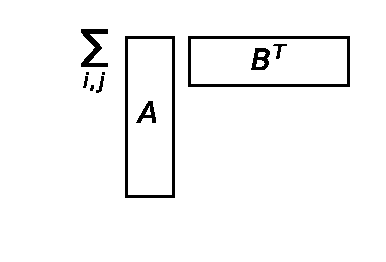
\includegraphics[width=130mm]{Results/normDifferenceFromUSVs.pdf}
\caption[Exact norm of difference]{Visualising the calculation of the norm of a difference via SVD's}
\label{fig:normDifferenceFromUSVs}
\end{figure}

\subsection{Decision Tree}
\label{sec:Introduction/Decision Tree}

There are several reasons for performing an SVD analysis. When applied to a single spatial field, it may be to find the PC's or EOF's, which describe areas that behave similarly. In many real-world applications, however, the analysis of a field does not only involve a single time period but includes data over multiple weeks, months or years. Then, researchers are interested in finding relevant patterns which appear in both datasets. The \textit{Maximum Covariance Analysis} (MCA) and \textit{Canonical Correlation Analysis} (CCA) examine the product matrix of two datasets and determine which patterns occur frequently and simultaneously~\cite{Eshel2011, Storch1999}. Such a pattern, or mode, is a combination of a left- and a right basis vector. One technique to determine these modes is to perform an SVD on the product of the standardised datasets. In some domains, the term SVD is used synonymously with MCA. In an MCA, modes are found where the left- and the right vector covary maximally, whereas in a CCA, they correlate maximally~\cite{Bretherton1992}.

\begin{figure}[H]
\centering
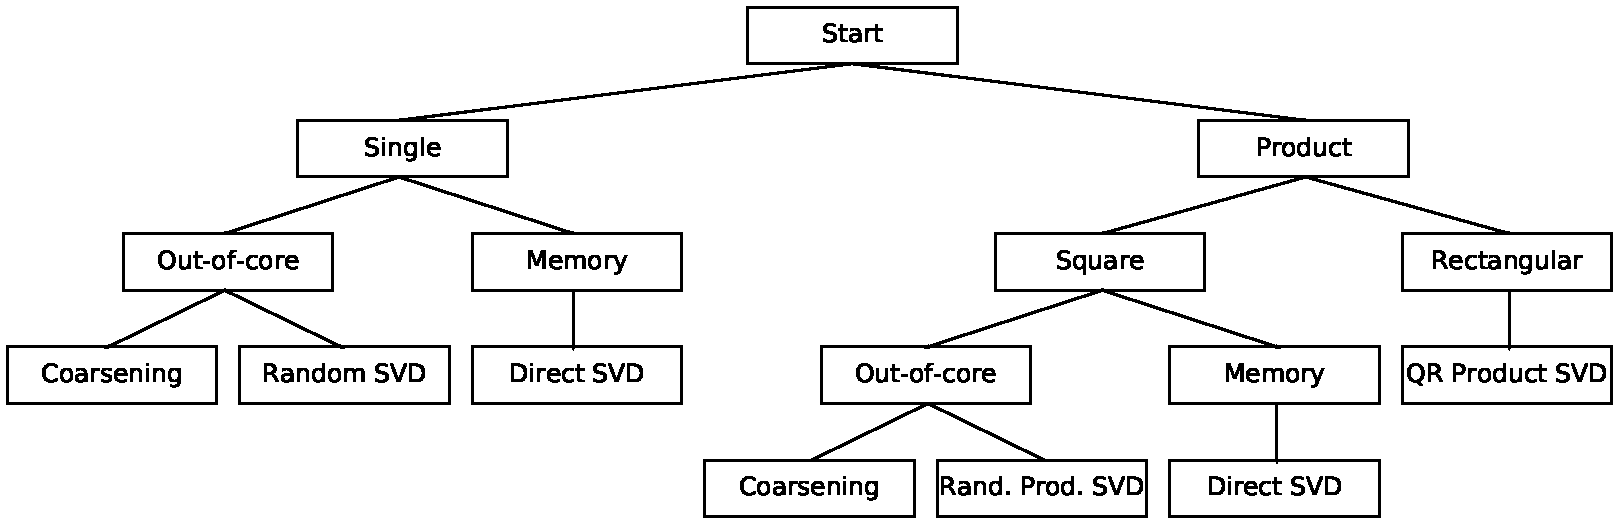
\includegraphics[width=\textwidth]{Results/FlowDiagram.pdf}
\caption{Decision tree describing the possible SVD techniques}
\label{fig:FlowDiagram}
\end{figure}

Figure~\ref{fig:FlowDiagram} shows several options a researcher has when performing an SVD. The first question to be answered is whether the SVD will be applied to a single matrix or to the product of two matrices. For single fields, the data may be small enough to fit in the memory of a computer. Then, a regular SVD is the best option. If the dataset is too large, two alternatives exists which provide an approximate answer. These will be discussed in section~\ref{sec:Results/Approximate SVD via Coarsening} and section~\ref{sec:Results/Approximate SVD via Dimensionality Reduction}.

When the SVD is performed on the product of two matrices, the best course of action depends on whether the matrices are square or rectangular. The rank of a matrix is at most the size of the smallest side, which, for rectangular matrices, can be small. How to exploit this fact is described in section~\ref{sec:Results/Exact Product SVD via QR Decomposition}. Square matrices small enough to fit in memory can be analysed directly. What to do with larger, square datasets is discussed in section~\ref{sec:Results/Approximate Product SVD via Coarsening} and section~\ref{sec:Results/Approximate Product SVD via Dimensionality Reduction}.

%%%%%%%%%%%%%%%%%%%%%%%%%%%%%%%%%%%%%%%%%%
\section{Materials and Methods}
\label{sec:Materials and Methods}

%Materials and Methods should be described with sufficient details to allow others to replicate and build on published results. Please note that publication of your manuscript implicates that you must make all materials, data, computer code, and protocols associated with the publication available to readers. Please disclose at the submission stage any restrictions on the availability of materials or information. New methods and protocols should be described in detail while well-established methods can be briefly described and appropriately cited.

%Research manuscripts reporting large datasets that are deposited in a publicly available database should specify where the data have been deposited and provide the relevant accession numbers. If the accession numbers have not yet been obtained at the time of submission, please state that they will be provided during review. They must be provided prior to publication.

%Interventionary studies involving animals or humans, and other studies require ethical approval must list the authority that provided approval and the corresponding ethical approval code. 

In domains such a climate science and phenology, datasets are typically spatio-temporal fields, e.g. of temperature. In such fields, values vary slowly and neighbouring points are not entirely independent of one another, neither in space nor in time~\cite{Eshel2011}. Then, there is a high level of autocorrelation and the field contains large scale structure. Such redundancy in the data means the matrix is rank deficient.

To compare our techniques and to establish a relation between performance and structure scale, we need to be able to generate fields which resemble those often encountered in real-world applications. Additionally, we require methods to measure the autocorrelation of fields.

\subsection{Spatio-Temporal Fields}
\label{sec:Materials and Methods/Spatio-Temporal Fields}

As simulated spatio-temporal fields, real-valued \textit{Gaussian Random Fields} (GRF's) are particularly useful because their structure scale can be captured in a single parameter. For such rotational invariant fields, the spectrum follows the power law described by $P(k) = c_{0} \, |\vec{k}|^{-\alpha}$ where $\vec{k}$ is the wavevector and~$\alpha$ the parameter which controls the level of autocorrelation. Figure~\ref{fig:GaussianRandomField} shows fields with various~$\alpha$'s.

\begin{figure}[H]
\centering
\subfloat[$\alpha = 1$]{\label{fig:GaussianRandomFieldSize400Alpha1.pdf}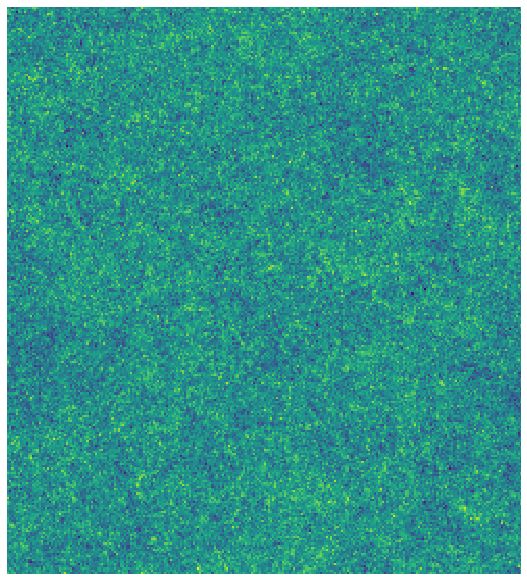
\includegraphics[scale=.4]{Results/GaussianRandomFieldSize400Alpha1.pdf}}
\hspace{8mm}
\subfloat[$\alpha = 3$]{\label{fig:GaussianRandomFieldSize400Alpha3.pdf}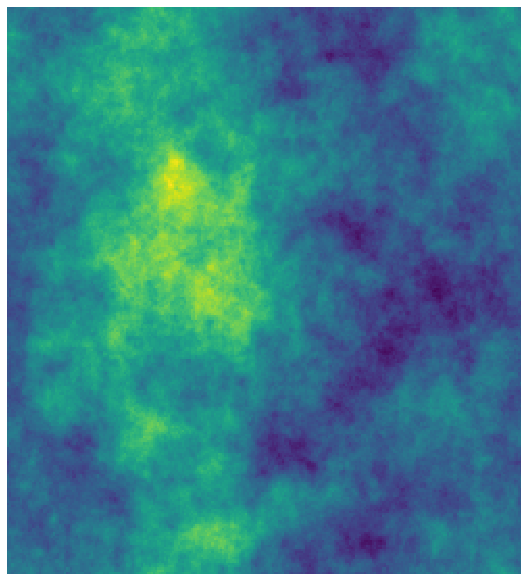
\includegraphics[scale=.4]{Results/GaussianRandomFieldSize400Alpha3.pdf}}
\hspace{8mm}
\subfloat[$\alpha = 5$]{\label{fig:GaussianRandomFieldSize400Alpha5.pdf}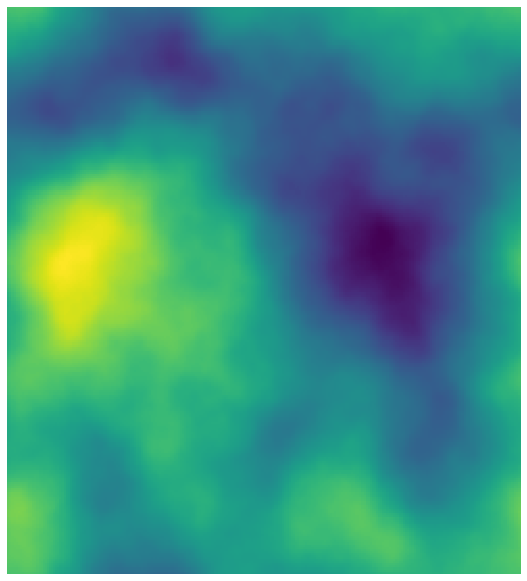
\includegraphics[scale=.4]{Results/GaussianRandomFieldSize400Alpha5.pdf}}
\caption{Gaussian Random Fields for various $\alpha$'s}
\label{fig:GaussianRandomField}
\end{figure}

Just as there is spatial autocorrelation, there is temporal autocorrelation, when the values of the field over the entire time period do not change drastically. In principle, there can be different levels of autocorrelation over time and over space. However, for simplicity, in this article we will use the same level of autocorrelation in all directions, determined by parameter~$\alpha$.

\subsection{Autocorrelation}
\label{sec:Materials and Methods/Autocorrelation}

In the geosciences, there are additional measures of spatial autocorrelation \cite{Eshel2011, Storch1999}. One frequently used is Moran's $I$~\cite{Moran1950, Hubert1981, PySAL}. Figure~\ref{fig:plotGammaAndMoransIAndBeta} shows the relationship between Moran's $I$, using a uniform kernel with a bandwidth equal to~$10$, and the $\alpha$ of our generated GRF's.

One can also devise an autocorrelation measure from the singular values of a dataset. Each singular value indicates the amount of variance explained by its associated mode. For fields with autocorrelation, the sorted list of singular values decays quickly. A power law can be fitted to this list, with an exponent which we call $\beta$. All three these measures provide an indication of the scale of the structure in the field and the level of autocorrelation in the data.

\begin{figure}[H]
\centering
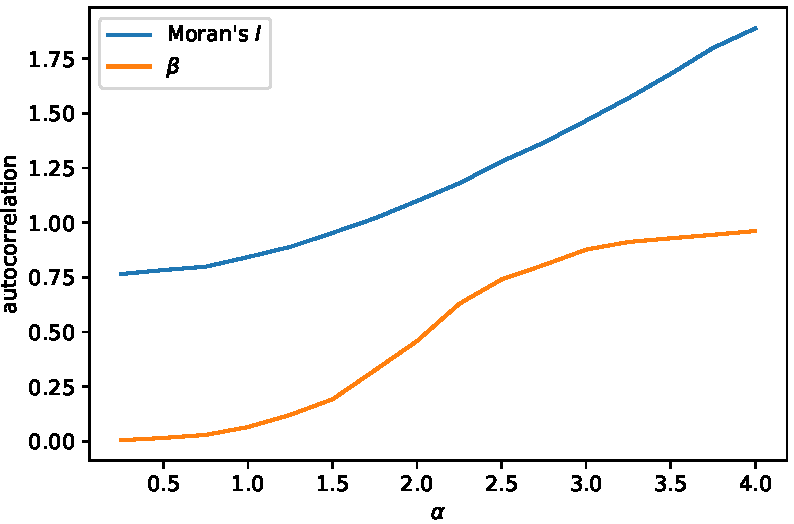
\includegraphics[width=80mm]{Results/plotMoransIAndBeta.pdf}
\caption[Various measures of autocorrelation]{Measures of autocorrelation as a function of $\alpha$}
\label{fig:plotGammaAndMoransIAndBeta}
\end{figure}

%%%%%%%%%%%%%%%%%%%%%%%%%%%%%%%%%%%%%%%%%%
\section{Results}

%This section may be divided by subheadings. It should provide a concise and precise description of the experimental results, their interpretation as well as the experimental conclusions that can be drawn.
%\begin{quote}
%This section may be divided by subheadings. It should provide a concise and precise description of the experimental results, their interpretation as well as the experimental conclusions that can be drawn.
%\end{quote}

This section lists several SVD related implementations to analyse large datasets efficiently by exploiting autocorrelation and rank deficiency. It includes three use cases to illustrate the procedures.

\subsection{Exact Product SVD via QR Decomposition}
\label{sec:Results/Exact Product SVD via QR Decomposition}

In real-world applications, researchers often wants to find the relation between two fields. Analyses such as the MCA and CCA, discussed in section~\ref{sec:Introduction/Decision Tree}, rely on performing an SVD of the product matrix of the two fields. Take two input datasets with the various spatial gridpoints as rows and the sample of recorded values over time as columns. Centring and multiplying these gives the cross-covariance matrix. For highly rectangular matrices, when there are many spatial gridpoints but few temporal samples, the resulting cross-covariance matrix is inefficiently large and obviously rank deficient. Performing a rank decomposition, such as the \textit{QR decomposition}, allows the SVD to be calculated in an efficient manner~\cite{Chan1982, Tygert2017}. Figure~\ref{fig:qrProductSVD} shows that the result is mathematically identical to the full SVD while no unnecessarily large, intermediate matrix is ever formed.

\begin{figure}[H]
\centering
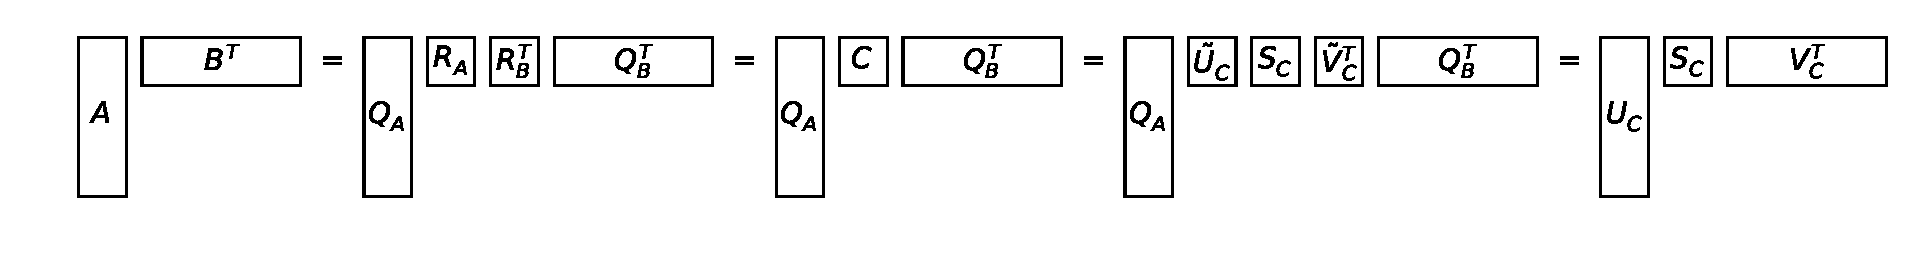
\includegraphics[width=\textwidth]{Results/qrProductSVD.pdf}
\caption[Exact SVD via QR decomposition]{Visualising the calculation of the exact SVD of a product via QR decomposition}
\label{fig:qrProductSVD}
\end{figure}

\subsection{Case Study using SI-x and AVHRR Data}
\label{sec:Results/Case Study using SI-x and AVHRR Data}

Let's apply the QR decomposition technique to phenological datasets. Phenology is the science that studies recurring biological events such as leafing and blooming as well as their causes and variations in space and time. Spatio-temporal fields of remotely sensed images can be used to derive various phenological metrics. One of these metrics is the so-called \textit{Start of Season} (SOS), which indicates the beginning of photosynthetic activity in plants. In this section, we use a SOS field of the US, made by processing time series of the \textit{Advanced Very High Resolution Radiometer} (AVHRR) sensor~\cite{Reed1994}. Additionally, we use the \textit{Extended Spring Indices} (SI-x), which are a suite of models that transform daily temperatures into consistent phenological metrics~\cite{Schwartz2013}. In particular, we take a version of the Bloom index which was recently generated for the US by adapting the SI-x models to a cloud computing environment~\cite{Izquierdo2015}. Both datasets span from $1989$ to $2014$ and have a $1\text{km}^2$ spatial resolution, meaning they are highly rectangular.

Clearly, these fields are not GRF's. Nonetheless, we can get an idea of their autocorrelation by estimating the $\alpha$ parameter. Calculated over a subsection of the US, we estimate the Bloom field to have $\alpha \approx 3.0$ and Moran's $I \approx 0.97$ and the SOS field to have $\alpha \approx 2.0$ and Moran's $I \approx 0.37$~\cite{Bogaardt2018}. These measures have no further influence on the SVD via QR decomposition because this technique provides an exact result. Indeed, the accompanying \textit{Jupyter Notebook}, as well as work being prepared for publication, shows that this technique provides the full SVD of the cross-covariance matrix in a matter of seconds, without ever exceeding the \textit{RAM}-memory~\cite{ZuritaMilla2018}.

\subsection{Approximate SVD via Coarsening}
\label{sec:Results/Approximate SVD via Coarsening}

As mentioned in section~\ref{sec:Introduction/Matrix Size and Rank}, real-world data are gathered by machines with finite precision. Realising that all fields contain some level of noise, it may not be necessary to determine the mathematically exact SVD. An approximation can provide an equivalent amount of information. Then, it is no longer \textit{efficient} to work with the full dataset, but it makes sense to reduce the data to the point where the error due to reduction is around the noise level.

When a spatial field has large scale structure, the values of neighbouring cells do not change drastically. Perhaps these cells can be aggregated together to produce a smaller dataset which still faithfully describes the original field. Here, we coarsen two dimensional GRF's.

\begin{figure}[H]
\centering
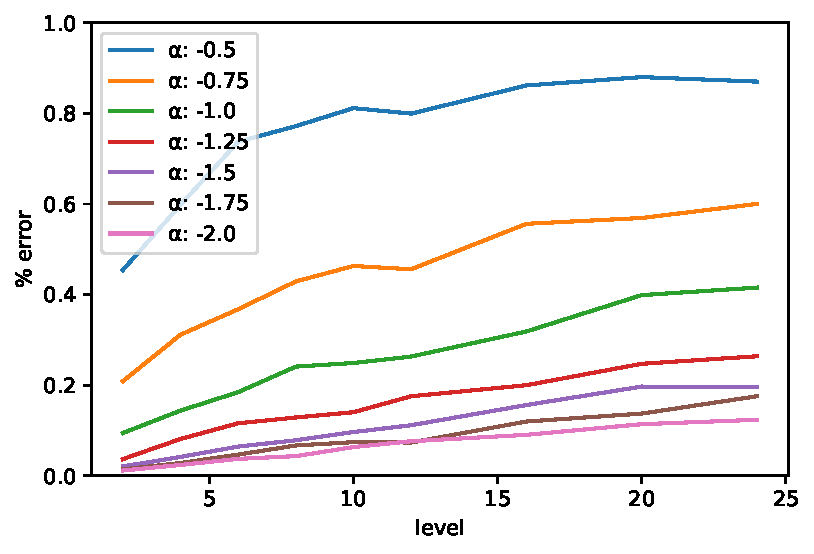
\includegraphics[width=80mm]{Results/plotSingleSpatialFieldViaCoarsening.pdf}
\caption[Error after coarsening]{Error in the SVD of a coarsened spatial field for various $\alpha$'s}
\label{fig:plotSingleSpatialFieldViaCoarsening}
\end{figure}

Figure~\ref{fig:plotSingleSpatialFieldViaCoarsening} shows the error in a coarsening process for matrices of various~$\alpha$'s and for different coarsening window sizes. The error is determined as the norm of the difference between the original matrix and the coarsened version, divided by the norm of the original~\cite{Bogaardt2018}. Other measures of similarity could have been used, such as the correlation between the two datasets, but this is left for future research. Note that a field with high autocorrelation, e.g. $\alpha=3$, differs by less than~$10\%$ from one~$25$ times smaller, at coarsening level~$5$.

\subsection{Approximate SVD via Dimensionality Reduction}
\label{sec:Results/Approximate SVD via Dimensionality Reduction}

An alternative methd of reducing the size of a matrix is via dimensionality reduction. For very large datasets, which do not fit in \textit{RAM}-memory and are saved out-of-core, reading the data becomes a major factor in determining the speed of the analysis~\cite{Halko2011}. An approximate rank decomposition of a large matrix can be obtained efficiently using a random algorithm~\cite{Halko2011, Li2016}. This procedure requires only a constant number of passes over the data, reducing storage reading time. The number of basis-vectors is, then, truncated to the~$l$ most important ones, similar to finding an $\epsilon$-rank approximation. The error can be made arbitrarily small by adjusting~$l$ and~$\epsilon$. Such dimensionality reduction discards modes which contribute little to the variance in a dataset.

\begin{figure}[H]
\centering
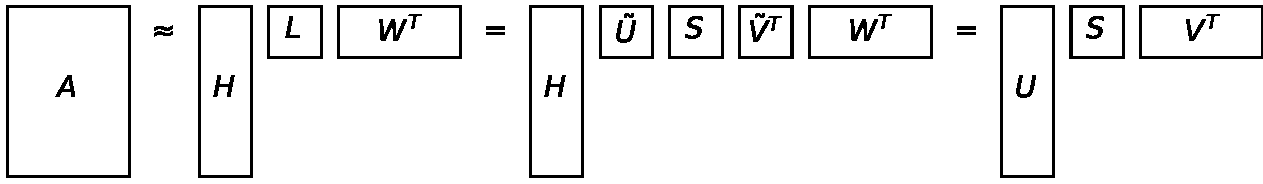
\includegraphics[width=100mm]{Results/reduceSizeRandomisedSquare.pdf}
\caption[Approximate randomised SVD]{Visualising the calculation of an approximate SVD via dimensionality reduction}
\label{fig:reduceSizeRandomisedSquare}
\end{figure}

Figure~\ref{fig:reduceSizeRandomisedSquare} depicts the calculation in this process, which first reduces the input matrix to a smaller square matrix of $l$~by~$l$. It also provides two projection matrices which can bring the rows and columns of this smaller matrix back to the bases of the original input. It is a randomised procedure to get an $\epsilon$-rank approximation and, therefore, the error is of the order of the size of the largest truncated singular value~\cite{Martinsson2016, Halko2011}. Subsequently, the SVD is applied to the small $l$~by~$l$ matrix, which results in a fast and efficient approximation of the matrix's decomposition.

As mentioned in section~\ref{sec:Introduction/Matrix Size and Rank}, an SVD is the procedure to obtain the best lower rank approximation~\cite{Eckart1936, Martinsson2016}. The calculations in the accompanying \textit{Jupyter Notebook} show that the errors induced by our randomised SVD procedure are negligible~\cite{Bogaardt2018}. The technique performs much better than coarsening. The coarsening procedure has several advantages though. For one, it is intuitive and the results are easy to interpret. It is also trivial to implement. Additionally, different coarsening levels can be applied to different directions. This is especially advantages when directions have different levels of autocorrelation or are recorded at different resolutions. Finally, the predictions of figure~\ref{fig:plotSingleSpatialFieldViaCoarsening} can help researchers determine at what resolution to gather their data in the first place. In domains were satellite data is used, datasets are often not very detailed because the imaging resolution is low. Unlike local analyses of developed countries, where high resolution data is becoming more accessible, for continental or global analyses, coarse spatial resolution data may simply be the only option.

\subsection{Case Study using ERA5 Data}
\label{sec:Results/Case Study using ERA5 Data}

\enlargethispage{4mm}
Coarsening and dimensionality reduction are particularly useful for spatial fields with high levels of autocorrelation. As an example of this, we examine humidity and cloud cover data from the ERA5 datasets for a single time period. ERA5 is an atmospheric reanalysis of the global climate using high spatial resolution forecasts, produced by combining models with observations~\cite{Dee2011}. It contains estimates of atmospheric parameters such as air temperature, pressure and wind at different altitudes.

The humidity field has a Moran's $I \approx 0.98$, while the cloud cover data shows less structure with a Moran's $I \approx 0.82$. The estimations for~$\alpha$ were unreliable, though figure~\ref{fig:plotGammaAndMoransIAndBeta} can help us translate the measures and suggests the fields are equivalent to GRF's with an $\alpha \sim 3.5$ and $\alpha \sim 2.5$, respectively. The coarsening predictions of figure~\ref{fig:plotSingleSpatialFieldViaCoarsening} indicate the first field should incur errors around a few percent for size reductions between~$2$ and~$8$, while the second field is expected to have errors between~$5\%$ and~$15\%$. The calculations in the accompanying \textit{Jupyter Notebook} show that this prediction is fairly accurate, perhaps slightly pessimistic. For the dimensionality reduction, the errors are completely negligible. If a researcher cares most about performance, dimensionality reduction is the best option.

\subsection{Approximate Product SVD via Coarsening}
\label{sec:Results/Approximate Product SVD via Coarsening}

While section~\ref{sec:Results/Approximate SVD via Coarsening} dealt with coarsening a single spatial field, we can also coarsen two fields before analysing their cross-covariance matrix. Figure~\ref{fig:plotProductSpatialTemporalFieldsViaCoarsening} shows the percentage error for various generated spatio-temporal fields. Note that only the two spatial directions are coarsened in our calculation. This is because the time direction gets eaten in the matrix product of the MCA or CCA and coarsening it will not speed up the SVD. Coarsening two spatial directions means each field is reduced by the square of the coarsening level, while the cross-covariance matrix is reduced by the level to the power~$4$. As a result, the typical error in this product is larger than for the single field, though the speed up is also substantial. Again, the level of autocorrelation plays an important part, with larger $\alpha$'s leading to less error. The amount of error likely also depends on the similarity between the two datasets, though we leave deeper investigation of this aspect for further research. 

\begin{figure}[H]
\centering
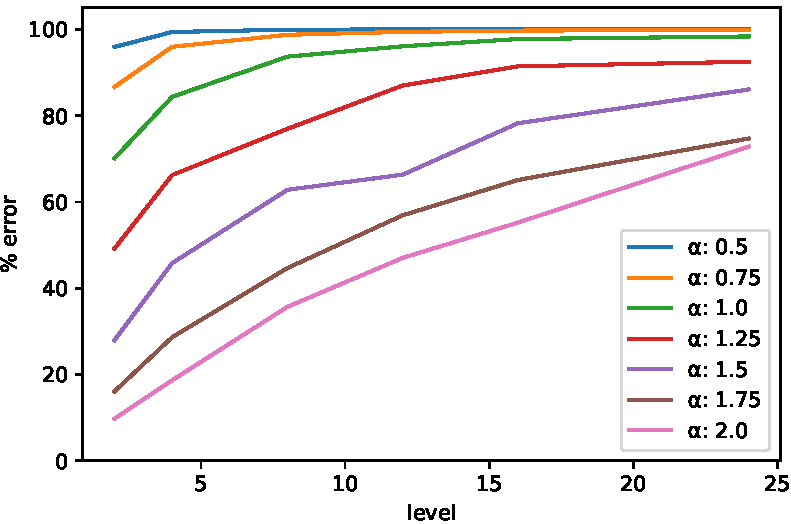
\includegraphics[width=80mm]{Results/plotProductSpatialTemporalFieldsViaCoarsening.pdf}
\caption[Error after coarsening]{Error in the SVD of the product of two coarsened fields for various $\alpha$'s}
\label{fig:plotProductSpatialTemporalFieldsViaCoarsening}
\end{figure}

\subsection{Approximate Product SVD via Dimensionality Reduction}
\label{sec:Results/Approximate Product SVD via Dimensionality Reduction}

The randomised dimensionality reduction process can be applied to two spatio-temporal fields before they are multiplied into the cross-covariance matrix. Similar to the QR decomposition of section~\ref{sec:Results/Exact Product SVD via QR Decomposition}, it has the advantage that the SVD is applied to a small $l$~by~$l$ matrix. This calculation is visualised in figure~\ref{fig:randomisedSquareProductSVD}.

\begin{figure}[H]
\centering
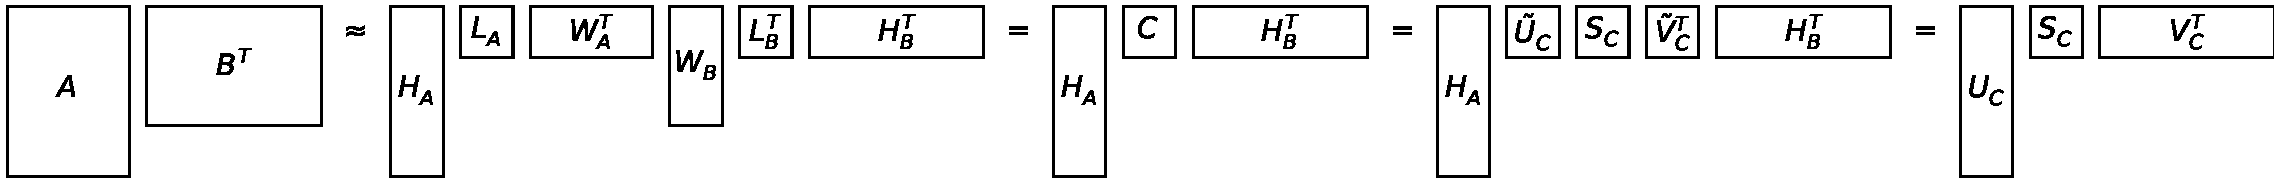
\includegraphics[width=\textwidth]{Results/randomisedSquareProductSVD.pdf}
\caption[Approximate product SVD]{Visualising the calculation of an approximate SVD for the product of two fields using dimensionality reduction}
\label{fig:randomisedSquareProductSVD}
\end{figure}

After generating various GRF's, the reduced cross-covariance matrix is compared with the original. Figure~\ref{fig:plotRandomisedSizeReducedMatrixProduct} shows that the results are quite bad for fields with a small $\alpha$, but high levels of autocorrelation allow for substantial savings in computation time without incurring much error. When performing an MCA or CCA on a spatio-temporal field, the spatial directions are flattened and some of the spatial autocorrelation is lost. This partially explains why the error is substantial for low $\alpha$. Again, we performed our analysis with two generated fields which correlated to some degree. Whether this correlation influences the amount of error after dimensionality reduction is left for further research.

\begin{figure}[H]
\centering
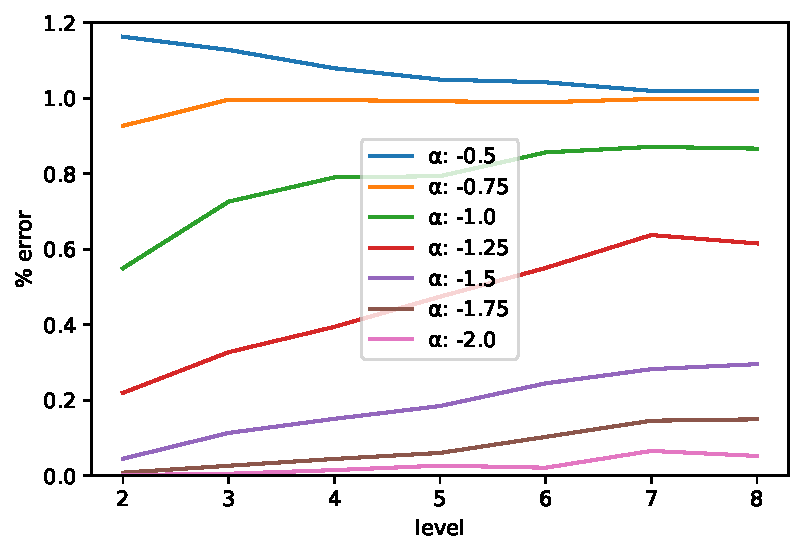
\includegraphics[width=80mm]{Results/plotRandomisedSizeReducedMatrixProduct.pdf}
\caption[Error after reduction]{Error in the SVD of the product of two reduced fields for various $\alpha$'s}
\label{fig:plotRandomisedSizeReducedMatrixProduct}
\end{figure}

The reduction of the number of dimensions of each input dataset before an MCA or CCA is actually advised by some researchers, as a method to filter out noise~\cite{Barnett1987}. Especially when the number of temporal samples is small, outliers and random fluctuations could affect the result~\cite{Bretherton1992}. This is because any statistical analysis will choose its regression-coefficients so as to optimize the fit. It may occur that two noise-vectors in the two fields coincidentally covary and show up as dominant modes. Prefiltering can alleviate this risk.

\subsection{Case Study using JRA55 Data}
\label{sec:Results/Case Study using JRA55 Data}

The JRA55 data is an atmosphere reanalysis product which includes quantities such as humidity, pressure and temperature~\cite{Kobayashi2015}. Recently, these quantities were used to determine the total meridional energy transport and latent heat, measures important to understand the global climate~\cite{Liu2018}. As an example of our reduction techniques for matrix products, we are using a Mercator projection of the energy transport and latent heat, recorded monthly from 1979 to 2015. Although the spatially flattened matrices are not completely square, their high resolution in the time direction make them substantially less rectangular than the phenology data from section~\ref{sec:Results/Case Study using SI-x and AVHRR Data}. Therefore, this serves as a good use case for the coarsening and dimensionality reduction techniques for a square product SVD.

The energy field has a Moran's $I \approx 0.93$, while the latent heat field has a Moran's $I \approx 0.86$. The estimations for~$\alpha$ were unreliable, though figure~\ref{fig:plotGammaAndMoransIAndBeta} can help us translate the measures and suggests the fields are equivalent to GRF's with an $\alpha \sim 3.0$ and $\alpha \sim 2.5$, respectively. The analyses of section~\ref{sec:Results/Approximate Product SVD via Coarsening} and of section~\ref{sec:Results/Approximate Product SVD via Dimensionality Reduction} showed that, for such~$\alpha$ levels, the errors should be quite high. In contrast, we found that coarsening the fields before applying an SVD on their product merely resulted in an error between $8\%$ and $16\%$. For the dimensionality reduction technique, as well, the predictions overstated the observed error, which were around a few percent, even for high levels of size reduction. 

%%%%%%%%%%%%%%%%%%%%%%%%%%%%%%%%%%%%%%%%%%
%\subsection{Subsection}

%\subsubsection{Subsubsection}

%Bulleted lists look like this:
%\begin{itemize}[leftmargin=*,labelsep=5.8mm]
%\item	First bullet
%\item	Second bullet
%\item	Third bullet
%\end{itemize}

%Numbered lists can be added as follows:
%\begin{enumerate}[leftmargin=*,labelsep=4.9mm]
%\item	First item 
%\item	Second item
%\item	Third item
%\end{enumerate}

%The text continues here.

%\subsection{Figures, Tables and Schemes}

%All figures and tables should be cited in the main text as Figure 1, Table 1, etc.

%\begin{figure}[H]
%\centering
%
\includegraphics[width=2 cm]{Definitions/logo-mdpi}
%\caption{This is a figure, Schemes follow the same formatting. If there are multiple panels, they should be listed as: (\textbf{a}) Description of what is contained in the first panel. (\textbf{b}) Description of what is contained in the second panel. Figures should be placed in the main text near to the first time they are cited. A caption on a single line should be centered.}
%\end{figure} 

%\begin{table}[H]
%\caption{This is a table caption. Tables should be placed in the main text near to the first time they are cited.}
%\centering
%% \tablesize{} %% You can specify the fontsize here, e.g. \tablesize{\footnotesize}. If commented out \small will be used.
%\begin{tabular}{ccc}
%\toprule
%\textbf{Title 1}	& \textbf{Title 2}	& \textbf{Title 3}\\
%\midrule
%entry 1		& data			& data\\
%entry 2		& data			& data\\
%\bottomrule
%\end{tabular}
%\end{table}

%\subsection{Formatting of Mathematical Components}

%This is an example of an equation:

%\begin{equation}
%a + b = c
%\end{equation}
%% If the documentclass option "submit" is chosen, please insert a blank line before and after any math environment (equation and eqnarray environments). This ensures correct linenumbering. The blank line should be removed when the documentclass option is changed to "accept" because the text following an equation should not be a new paragraph. 

%Please punctuate equations as regular text. Theorem-type environments (including propositions, lemmas, corollaries etc.) can be formatted as follows:
%% Example of a theorem:
%\begin{Theorem}
%Example text of a theorem.
%\end{Theorem}

%The text continues here. Proofs must be formatted as follows:

%% Example of a proof:
%\begin{proof}[Proof of Theorem 1]
%Text of the proof. Note that the phrase `of Theorem 1' is optional if it is clear which theorem is being referred to.
%\end{proof}
%The text continues here.

%%%%%%%%%%%%%%%%%%%%%%%%%%%%%%%%%%%%%%%%%%
\section{Discussion}

%Authors should discuss the results and how they can be interpreted in perspective of previous studies and of the working hypotheses. The findings and their implications should be discussed in the broadest context possible. Future research directions may also be highlighted.

\subsection{Further Work}
\label{sec:Discussion/Further Work}

Much of the analysis here relies on a priori knowledge of the level of autocorrelation. The \textit{Jupyter Notebook} accompanying this article includes an algorithm which estimates Moran's $I$ based on a sample of gridpoints. This speeds up the calculation substantially for large datasets. Additional work could be placed into making this algorithm more professional and more user friendly. It would also be an improvement to relax the assumption that the autocorrelation in the time direction is similar to that in the spatial directions. In fact, it is more realistic to allow for different levels of autocorrelation in all directions and to have a version of Moran's $I$ which can estimate these values.

Furthermore, note that, unlike the coarsening procedure, the dimensionality reduction is not applied on each spatial field for each time period, but rather on the entire spatially flattened timeseries. Therefore, the level of spatial autocorrelation may not be as important as the level of temporal autocorrelation. Further work can examine how to apply the reduction to the spatial part of the spatio-temporal fields, before it is flattened. Alternative solutions, which retain the spatial structure, may include 3D tensor operations such as \textit{Higher-Order Singular Value Decomposition} (HOSVD)~\cite{Tucker1964}.

Finally, a warning about autocorrelation and standardisation. In MCA's, the timeseries of each spatial gridpoint is centred about its mean and in CCA's, each gridpoint is standardised. This operation destroys much of the spatial autocorrelation, as it can affect neighbouring cells differently. Determining the level of autocorrelation, e.g. by calculating Moran's $I$, should be done after the preprocessing steps. 

\subsection{Summary}
\label{sec:Discussion/Summary}

In summary, randomised dimensionality reduction works best for datasets which are too large for internal memory. Performing analyses at a coarse level can be beneficial when data collection is difficult. These techniques require at least some autocorrelation in the fields, which results in rank deficient datasets. %\footnote{In the \textit{Jupyter Notebook} accompanying this article, we applied the techniques to real datasets of phenological metrics and obtained similar results to those predicted by the Gaussian Random Fields~\cite{Bogaardt2018}.}
% and when different directions have different levels of autocorrelation.
In general, rank decompositions can speed up calculations by splitting datasets into smaller, square matrices of full rank. Once the analysis is performed on the smaller matrix, the output can be rotated back to the original bases, saving memory usage and computation time.

%%%%%%%%%%%%%%%%%%%%%%%%%%%%%%%%%%%%%%%%%%
%\section{Conclusions}

%This section is not mandatory, but can be added to the manuscript if the discussion is unusually long or complex.

%%%%%%%%%%%%%%%%%%%%%%%%%%%%%%%%%%%%%%%%%%
%\section{Patents}
%This section is not mandatory, but may be added if there are patents resulting from the work reported in this manuscript.

%%%%%%%%%%%%%%%%%%%%%%%%%%%%%%%%%%%%%%%%%%
\vspace{6pt} 

%%%%%%%%%%%%%%%%%%%%%%%%%%%%%%%%%%%%%%%%%%
%% optional
%\supplementary{The following are available online at \linksupplementary{s1}, Figure S1: title, Table S1: title, Video S1: title.}

% Only for the journal Methods and Protocols:
% If you wish to submit a video article, please do so with any other supplementary material.
% \supplementary{The following are available at \linksupplementary, Figure S1: title, Table S1: title, Video S1: title. A supporting video article is available at doi: link.}

%%%%%%%%%%%%%%%%%%%%%%%%%%%%%%%%%%%%%%%%%%
\authorcontributions{Conceptualization, R.Z.; Methodology, L.B.; Software, L.B.; Validation, R.G., R.Z. and E.I.; Formal Analysis, L.B.; Investigation, L.B.; Resources, R.G., R.Z. and E.I.; Data Curation, R.G., R.Z. and E.I.; Writing—Original Draft Preparation, L.B.; Writing—Review \& Editing, R.G., R.Z. and E.I.; Visualization, L.B.; Supervision, R.G. and R.Z.; Project Administration, R.G.; Funding Acquisition, R.Z.}

%%%%%%%%%%%%%%%%%%%%%%%%%%%%%%%%%%%%%%%%%%
\funding{This research was funded by the Nederlandse Organisatie voor Wetenschappelijk Onderzoek (NWO).}

%%%%%%%%%%%%%%%%%%%%%%%%%%%%%%%%%%%%%%%%%%
%\acknowledgments{In this section you can acknowledge any support given which is not covered by the author contribution or funding sections. This may include administrative and technical support, or donations in kind (e.g. materials used for experiments).}

%%%%%%%%%%%%%%%%%%%%%%%%%%%%%%%%%%%%%%%%%%
\conflictsofinterest{The authors declare no conflict of interest. The founding sponsors had no role in the design of the study; in the collection, analyses, or interpretation of data; in the writing of the manuscript, and in the decision to publish the results.} 

%%%%%%%%%%%%%%%%%%%%%%%%%%%%%%%%%%%%%%%%%%
%% optional
\abbreviations{The following abbreviations are used in this manuscript:\\

\noindent 
\begin{tabular}{@{}ll}
SVD & Singular value decomposition\\
GRF & Gaussian random field\\
PC & Principle component\\
EOF & Empirical orthogonal function\\
SOS & Start of season\\
SI-x & Extended spring indices\\
AVHRR & Advanced very-high-resolution radiometer\\
ERA5 & European fifth generation reanalysis\\
JRA55 & Japanese 55-year reanalysis\\
HOSVD & Higher-order singular value decomposition
\end{tabular}}

%%%%%%%%%%%%%%%%%%%%%%%%%%%%%%%%%%%%%%%%%%
%% optional
%\appendixtitles{no} %Leave argument "no" if all appendix headings stay EMPTY (then no dot is printed after "Appendix A"). If the appendix sections contain a heading then change the argument to "yes".
%\appendixsections{multiple} %Leave argument "multiple" if there are multiple sections. Then a counter is printed ("Appendix A"). If there is only one appendix section then change the argument to "one" and no counter is printed ("Appendix").
%\appendix
%\section{}
%\subsection{}
%The appendix is an optional section that can contain details and data supplemental to the main text. For example, explanations of experimental details that would disrupt the flow of the main text, but nonetheless remain crucial to understanding and reproducing the research shown; figures of replicates for experiments of which representative data is shown in the main text can be added here if brief, or as Supplementary data. Mathematical proofs of results not central to the paper can be added as an appendix.

%\section{}
%All appendix sections must be cited in the main text. In the appendixes, Figures, Tables, etc. should be labeled starting with `A', e.g., Figure A1, Figure A2, etc. 

%%%%%%%%%%%%%%%%%%%%%%%%%%%%%%%%%%%%%%%%%%
% Citations and References in Supplementary files are permitted provided that they also appear in the reference list here. 

%=====================================
% References, variant A: internal bibliography
%=====================================
%\reftitle{References}
%\begin{thebibliography}{999}
% Reference 1
%\bibitem[Author1(year)]{ref-journal}
%Author1, T. The title of the cited article. {\em Journal Abbreviation} {\bf 2008}, {\em 10}, 142-149, DOI.
% Reference 2
%\bibitem[Author2(year)]{ref-book}
%Author2, L. The title of the cited contribution. In {\em The Book Title}; Editor1, F., Editor2, A., Eds.; Publishing House: City, Country, 2007; pp. 32-58, ISBN.
%\end{thebibliography}

% The following MDPI journals use author-date citation: Arts, Econometrics, Economies, Genealogy, Humanities, IJFS, JRFM, Laws, Religions, Risks, Social Sciences. For those journals, please follow the formatting guidelines on http://www.mdpi.com/authors/references
% To cite two works by the same author: \citeauthor{ref-journal-1a} (\citeyear{ref-journal-1a}, \citeyear{ref-journal-1b}). This produces: Whittaker (1967, 1975)
% To cite two works by the same author with specific pages: \citeauthor{ref-journal-3a} (\citeyear{ref-journal-3a}, p. 328; \citeyear{ref-journal-3b}, p.475). This produces: Wong (1999, p. 328; 2000, p. 475)

%=====================================
% References, variant B: external bibliography
%=====================================
\externalbibliography{yes}
\bibliography{Bibliography}

%%%%%%%%%%%%%%%%%%%%%%%%%%%%%%%%%%%%%%%%%%
%% optional
%\sampleavailability{Samples of the compounds ...... are available from the authors.}

%% for journal Sci
%\reviewreports{\\
%Reviewer 1 comments and authors’ response\\
%Reviewer 2 comments and authors’ response\\
%Reviewer 3 comments and authors’ response
%}

%%%%%%%%%%%%%%%%%%%%%%%%%%%%%%%%%%%%%%%%%%
\end{document}

